\chapter{Μέθοδοι \tl{LQG} εγγυημένου κόστους}\label{ch:gcc}
Στο σημείο αυτό θα παρουσιάσουμε τον εύρωστο έλεγχο γραμμικών αβέβαιων
συστημάτων με τετραγωνικό δείκτη συμπεριφοράς στο πλαίσιο του ελέγχου εγγυημένου
κόστους. Η ανάπτυξη που θα ακολουθήσει βασίστηκε στο
βιβλίο~\cite{kosmidou2009robust}. Ο ενδιαφερόμενος παραπέμπεται στο
συγκεκριμένο καθώς θα παρουσιάσουμε μονάχα κάποια βασικά αποτελέσματα, χωρίς τις
αντίστοιχες αποδείξεις, αλλά θα επικεντρωθούμε στην υλοποίηση των μεθόδων μέσω
παραδειγμάτων με τη βοήθεια του \tl{MATLAB}.

Ένα τυπικό γραμμικό αβέβαιο σύστημα είναι της μορφής
\begin{equation}\label{eq:un_ss}
    \dot{x}(t) = (A + \Delta A)x(t) + (B + \Delta B) u(t), \quad x(0) = x_0,
\end{equation}
για \( t \geq 0 \), όπου \( x(t) \in \mathbb{R}^n \) το διάνυσμα κατάστασης,
\( u(t) \in \mathbb{R}^m \) το διάνυσμα ελέγχου, \( A \) και \( B \) οι πίνακες
κατάστασης και ελέγχου αντίστοιχα, κατάλληλων διαστάσεων. Οι αβεβαιότητες περιγράφονται
με τη μορφή γραμμικών συναρτήσεων
\[
    \Delta A = \sum_{i = 1}^{k} A_i r_i, \quad
    \Delta B = \sum_{i = 1}^{l} B_i p_i,
\]
όπου \( A_i \) και \( B_i \) είναι σταθεροί πίνακες και \( r_i, p_i \) βαθμωτά
μεγέθη, που μπορεί να είναι και χρονικά μεταβαλλόμενα στη γενική περίπτωση. Με
την παραπάνω περιγραφή ορίζουμε τα σύνολο
\begin{align*}
    \mathcal{R} &:= \{ r \in \mathbb{R}^k: |r_i| \leq \bar{r}, \bar{r} > 0, ,i = 1, \dots,
    k \} \\
    \mathcal{J} &:= \{ p \in \mathbb{R}^p: |p_i| \leq \bar{p}, \bar{p} > 0, ,i = 1, \dots,
    l \}.
\end{align*}
Χωρίς να μειωθεί η γενικότητα τα όρια μπορούν να κανονικοποιηθούν, δηλαδή \(
\bar{r} = \bar{p} = 1 \). Έτσι ονομάζουμε \emph{αποδεκτή αβεβαιότητα}, τις
αβεβαιότητες που ικανοποιούν τις γραμμικές μορφές, όπως ορίστηκαν παραπάνω, και
βρίσκονται εντός των φραγμένων συνόλων.

Στόχος είναι να βρεθεί γραμμικός νόμος ελέγχου με ανάδραση κατάστασης σταθερού
κέρδους, έτσι ώστε το κλειστό σύστημα να διατηρεί την ασυμπτωτική ευστάθεια και
ένα επιθυμητό επίπεδο επιδόσεων, για κάθε αποδεκτή αβεβαιότητα.

Θα θεωρήσουμε τις επιδόσεις του συστήματος ότι περιγράφονται από τετραγωνική
συνάρτηση κόστους
\begin{equation}\label{eq:un_cost}
    J(x_0, \Delta A, \Delta B, t) = \int_0^{\infty}
    \left[ x^T(t)Qx(t) + u^T(t)Ru(t) \right] \, dt,
\end{equation}
με \( Q \geq 0 \) και \( R > 0 \) όπου θέλουμε να ελαχιστοποιήσουμε. Για να το
επιτύχουμε αυτό υποθέτουμε ότι το ζεύγος \( (A, B) \) είναι ελέγξιμο και το
ζεύγος \( (Q^{1/2}, A) \) είναι παρατηρήσιμο. Ακόμη θεωρούμε το διάνυσμα
κατάστασης είναι διαθέσιμο προς μέτρηση. Στην περίπτωση που δεν υπάρχουν
αβεβαιότητες το πρόβλημα συμπίπτει με το πρόβλημα του γραμμικού τετραγωνικού ρυθμιστή.

Για το σύστημα~\eqref{eq:un_ss} με την τετραγωνική συνάρτηση κόστους
\eqref{eq:un_cost} η συνάρτηση \( \tilde{u}:\mathbb{R} \to \mathbb{R}^m \)
ονομάζεται \emph{νόμος ελέγχου εγγυημένου κόστους}, αν υπάρχει ένας θετικός
αριθμός \( \tilde{J} \), που λέγεται \emph{εγγυημένο κόστος}, τέτοιος ώστε
\[
    J(x_0, \tilde{u}, \Delta A, \Delta B, t) \leq \tilde{J}
\]
για όλες τις αποδεκτές αβεβαιότητες. Αποδεικνύεται ότι ο γραμμικός νόμος ελέγχου
ανάδρασης κατάστασης
\begin{equation}\label{eq:un_u_tilde}
    \tilde{u}(t) = Kx(t) = - R^{-1}B^{T}Px(t),
\end{equation}
είναι ένας νόμος ελέγχου εγγυημένου κόστους και
\[
    \tilde{J}(x_0) = x_0^{T}Px_0,
\]
είναι ένα εγγυημένο κόστος ή με κάποιες τεχνικές παραδοχές στην αντίστοιχη μορφή
\begin{equation}\label{eq:un_gcc_J}
    \tilde{J} = \tr{P},
\end{equation}
αν υπάρχει ένας θετικά ορισμένος συμμετρικός πίνακας
\( P \) που ικανοποιεί τη γενικευμένη αλγεβρική εξίσωση \tl{Riccati}, για
συντομία \tl{GARE},
\begin{equation}\label{eq:un_gare_general}
    PA + A^{T}P - PBR^{-1}B^{T}P + Q + \mathcal{U}(P) = 0.
\end{equation}
Η συνάρτηση \( \mathcal{U}(P) \) είναι μία συνάρτηση άνω φράγματος που εξαρτάται
από τις αβεβαιότητες και ισχύει
\begin{equation}\label{eq:un_bound}
    2x^T(t)P\Delta Ax(t) + 2 x^T(t)P\Delta BKx(t) \leq x^T(t)\mathcal{U}(P)x(t),
\end{equation}
για κάθε \( x \) και για όλες τις αποδεκτές αβεβαιότητες.

\section{Συστήματα με αβεβαιότητα στον πίνακα κατάστασης}
Στην περίπτωση αυτή έχουμε αβεβαιότητα μόνο στον πίνακα κατάστασης, δηλαδή
έχουμε \( \Delta B = 0 \). Έτσι για το άνω φράγμα \( \mathcal{U}(P) \), η
σχέση~\eqref{eq:un_bound} θα γίνει
\begin{equation}\label{eq:un_bound_linear}
    P\Delta A + \Delta A^{T}P \leq \mathcal{U}.
\end{equation}
Τότε διακρίνουμε δύο περιπτώσεις φράγματος,
\begin{enumerate} [label = (\enumgreek*)]
    \item φράγμα με βάση τις ιδιοτιμές,
    \item γραμμικό φράγμα.
\end{enumerate}

\subsection{Φράγμα με βάση τις ιδιοτιμές}
Στην περίπτωση αυτή, εφόσον ο πίνακας στο αριστερό μέλος της
σχέσης~\eqref{eq:un_bound_linear} είναι συμμετρικός, υπάρχουν ορθογώνιοι
πίνακες μετασχηματισμού \( M_i \) τέτοιοι ώστε
\[
    M_i^{T}(PA_i + A_i^{T}P)M_i = \Lambda_i,
\]
όπου \( \Lambda_i \) διαγώνιοι πίνακες. Αν συμβολίσουμε με \( |\Lambda_i| \)
τους αντίστοιχους πίνακες όπου τα διαγώνια στοιχεία έχουν αντικατασταθεί από τις
απόλυτες τιμές, τότε μία συνάρτηση άνω φράγματος που ικανοποιεί
την~\eqref{eq:un_bound_linear} είναι
\[
    \mathcal{U}(P) = \sum_{i = 1}^{k}M_i|\Lambda_i|M_i^{T}.
\]
Με αντικατάσταση της παραπάνω \( \mathcal{U}(P) \) στη γενικευμένη αλγεβρική
εξίσωση \tl{Riccati}~\eqref{eq:un_gare_general}, μπορούμε να υπολογίσουμε το
πίνακα \( P \). Στη συνέχεια από τη σχέση~\eqref{eq:un_u_tilde} βρίσκουμε το
νόμο ελέγχου εγγυημένου κόστους και το αντίστοιχο εγγυημένο κόστος από τη
σχέση~\eqref{eq:un_gcc_J}. Παρόλο που η τεχνική είναι εφικτή από θεωρητική
σκοπιά, πρακτικά είναι δύσκολα εφαρμόσιμη. Ακόμη δεν υπάρχει απόδειξη σύγκλισης
ούτε και συνθήκη ύπαρξης θετικά ορισμένης λύσης \( P \).

\subsection{Γραμμικό φράγμα}
Στην περίπτωση αυτή αποδεικνύεται ότι, για το αριστερό
μέλος της σχέσης~\eqref{eq:un_bound_linear} ισχύει η ανισότητα
\[
    P\Delta A + \Delta A^{T}P \leq P\Gamma P + \sum_{i = 1}^{k}A_i^{T}\Gamma^{-1}A_i.
\]
Αν επιλέξουμε \( \Gamma = \varepsilon P^{-1} \) τότε μπορούμε να επιλέξουμε σαν
συνάρτηση άνω φράγματος
\begin{equation}\label{eq:gcc_u_linear}
    \mathcal{U}(P) = k\varepsilon P + \varepsilon^{-1}\sum_{i = 1}^{k}A_i^{T}PA_i.
\end{equation}
Έτσι λαμβάνουμε μία συνάρτηση άνω φράγματος γραμμική ως προς τον πίνακα
\( P \). Ακόμα μέση της παραμέτρου \( \varepsilon \) μπορούμε να ικανοποιήσουμε
περαιτέρω προδιαγραφές σχεδίασης, με μία πιθανή επιλογή της παραμέτρου να είναι
\( \varepsilon = \sum \| A_i \| \) ώστε να εισαχθεί ένα μέτρο του μεγέθους της
αβεβαιότητας. Τέλος η παράμετρος \( k \) που πολλαπλασιάζει τον πρώτο όρο της
παραπάνω σχέσης, επιλέγεται έτσι ώστε να μηδενίζει τη συνάρτηση φράγματος όταν
δεν υπάρχουν αβεβαιότητες.

Αντικαθιστώντας τη συνάρτηση άνω φράγματος~\eqref{eq:gcc_u_linear} στη
γενικευμένη αλγεβρική εξίσωση \tl{Riccati}~\eqref{eq:un_gare_general}, τότε
προκύπτει μία μη γραμμική αλγεβρική εξίσωση της μορφής \( f(x) = 0 \). Μία
διαδεδομένη μέθοδος για την επίλυση τέτοιων εκφράσεων είναι με τη μέθοδο
\tl{Newton} (ή \tl{Newton-Raphson}). Η σχέση~\eqref{eq:un_gare_general}, είναι
μία σχέση πινάκων, διάστασης \( n \times n \), όπου \( n \) η διάσταση του
διανύσματος κατάστασης. Επομένως για να εφαρμόσουμε τη μέθοδο \tl{Newton}
πρέπει να μετατρέψουμε την~\eqref{eq:un_gare_general} σε διανυσματική. Ακόμα με
τη συνάρτηση \mono{fsolve} του \tl{MATLAB}, που υλοποιεί τη μέθοδο
\tl{Newton-Raphson} υπολογίζουμε τελικά τον θετικά
ορισμένο πίνακα \( P \). Στη συνέχεια από τη σχέση~\eqref{eq:un_u_tilde}
βρίσκουμε το νόμο ελέγχου εγγυημένου κόστους και το αντίστοιχο εγγυημένο
κόστος από τη σχέση~\eqref{eq:un_gcc_J}.

Ένα γνωστό πρόβλημα της μεθόδου \tl{Newton-Raphson} είναι ότι η σύγκλιση και
η επιτυχία της μεθόδου εξαρτάται από την αρχική εκτίμηση. Μία λογική αρχική
εκτίμηση για την εκκίνηση της μεθόδου είναι ο πίνακας \( P \) που υπολογίζεται
λύνοντας την αλγεβρική εξίσωση \tl{Riccati}. Δηλαδή η λύση αν το σύστημα δεν
ήταν αβέβαιο. Όπως παρατηρήσαμε στην πράξη, αυτή η αρχική εκτίμηση είναι αρκετά
καλή καθώς παρουσιάστηκε σύγκλιση σε οποιοδήποτε παράδειγμα επιλύσαμε. Φυσικά
στη συγκεκριμένη εργασία θα παρουσιάσουμε ένα μονάχα παράδειγμα για τη
συγκεκριμένη τεχνική.

Θα εφαρμόσουμε τη παραπάνω διαδικασία σε ένα παράδειγμα. Το παράδειγμα που θα
παρουσιάσουμε είναι απλό και έχει εσκεμμένα επιλεγεί έτσι για ευκολότερη κατανόηση.
Παρόλα αυτά η σχεδίαση του κώδικα έχει γραφτεί με το σκεπτικό να επιλύει οποιοδήποτε
πρόβλημα εισάγουμε.

Έστω το σύστημα
\[
    \dot{x} = Ax + Bu,
\]
όπου οι πίνακες \( A \) και \( B \) είναι
\[
    A =
    \begin{bmatrix}
        -1 & 0 \\
        1 & -2
    \end{bmatrix}, \quad
    B = \begin{bmatrix}0 \\ 1\end{bmatrix}.
\]
Τα μητρώα στάθμισης του δείκτη απόδοσης, σχέση~\eqref{eq:un_cost}, επιλέχθηκαν
\( Q = I_3 \) και \( R = 10 \). Ακόμα οι αβεβαιότητες στον πίνακα κατάστασης
επιλέχθηκαν
\[
    A_1(r_1) =
    r_1\begin{bmatrix}
        0 & 0 \\
        3 & 0
    \end{bmatrix}, \quad
    A_2(r_2) =
    r_2\begin{bmatrix}
        0 & 0 \\
        0 & 1.5
    \end{bmatrix}.
\]
Η σχέση~\eqref{eq:gcc_u_linear} μπορεί να γραφτεί στην ισοδύναμη μορφή
\[
    \mathcal{U}(P) = \varepsilon P + \varepsilon^{-1}\Delta A^{T}P\Delta A,
\]
καθώς υπάρχουν αβεβαιότητες. Έτσι η γενικευμένη αλγεβρική εξίσωση \tl{Riccati}
θα γίνει
\begin{equation}\label{eq:un_gare_linear}
    PA + A^{T}P - PBR^{-1}B^{T}P + Q + \varepsilon P +
    \varepsilon^{-1}\Delta A^{T}P\Delta A = 0.
\end{equation}
Στο παράδειγμα επιλέξαμε την παράμετρο
\( \varepsilon = 1 \) και δίχως μείωση της γενικότητας βρήκαμε το εγγυημένο
κόστος για τα κανονικοποιημένα όρια των αποδεκτών αβεβαιοτήτων, δηλαδή για
\( |r_1| \leq 1 \) και \( |r_2| \leq 1 \).

Τελικά, βρίσκουμε τον πίνακα \( P \) της γενικευμένης αλγεβρικής εξίσωσης
\tl{Riccati}
\[
    P =
    \begin{bmatrix}
        16.5034 & 3.0037 \\
        3.0037 & 1.1554
    \end{bmatrix},
\]
που είναι συμμετρικός και θετικά ορισμένος με ιδιοτιμές
\( \lambda_{1, 2} = 0.5884, 17.0703 \). Από τη σχέση~\eqref{eq:un_u_tilde}
ο νόμος ελέγχου εγγυημένου κόστους υπολογίζεται
\[
    \tilde{u}(t) = - R^{-1}B^{T}Px(t) =
    \begin{bmatrix}
        -0.3004 & -0.1155
    \end{bmatrix}x(t).
\]
Το εγγυημένο κόστος υπολογίζεται από τη σχέση~\eqref{eq:un_gcc_J}
\[
    \tilde{J} = \tr{P} = 17.6587,
\]
ενώ από τη σχέση που εξαρτάται από τις αρχικές συνθήκες
\[
    \tilde{J}(x_0) = x_0^{T}Px_0 =
    \begin{bmatrix}
        1 & 2
    \end{bmatrix}P
    \begin{bmatrix}
        1 & 2
    \end{bmatrix}^T = 33.1396.
\]
Στα σχήματα~\ref{fig:gcc_linear_bound1},~\ref{fig:gcc_linear_bound2}
και~\ref{fig:gcc_linear_bound3} παρουσιάζονται οι καταστάσεις του συστήματος για
τις διάφορες τιμές των αβεβαιοτήτων καθώς και ο νόμος ελέγχου εγγυημένου
κόστους.
\begin{figure}[h]
    \centering
    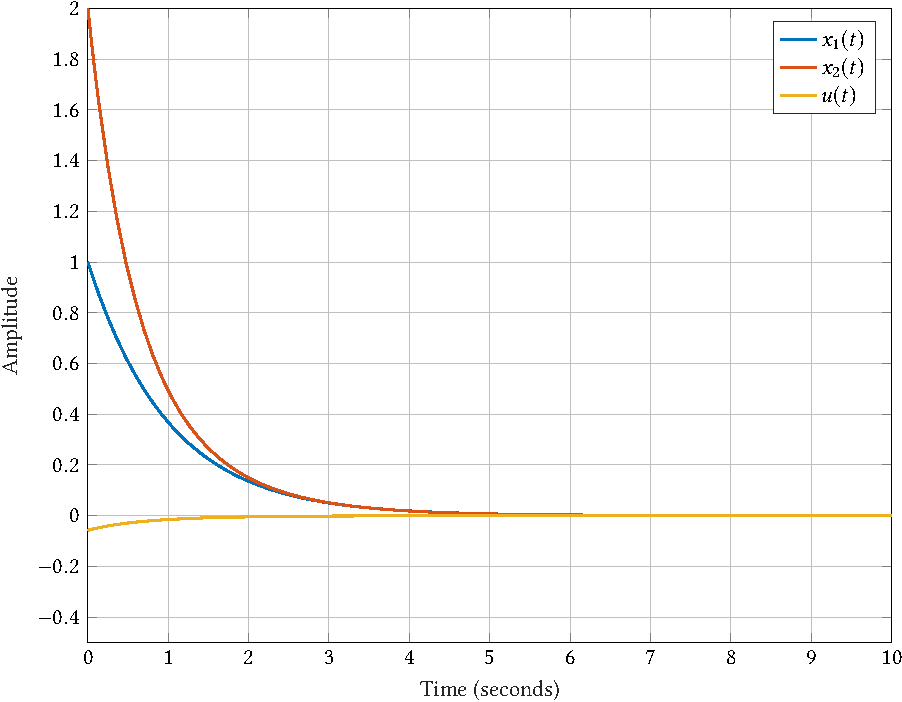
\includegraphics[width=0.9\textwidth]{figures/gcc_linear_bound1.pdf}
    \captionG{Αρχικό σύστημα χωρίς αβεβαιότητες}
    \label{fig:gcc_linear_bound1}
\end{figure}
\begin{figure}[h]
    \centering
    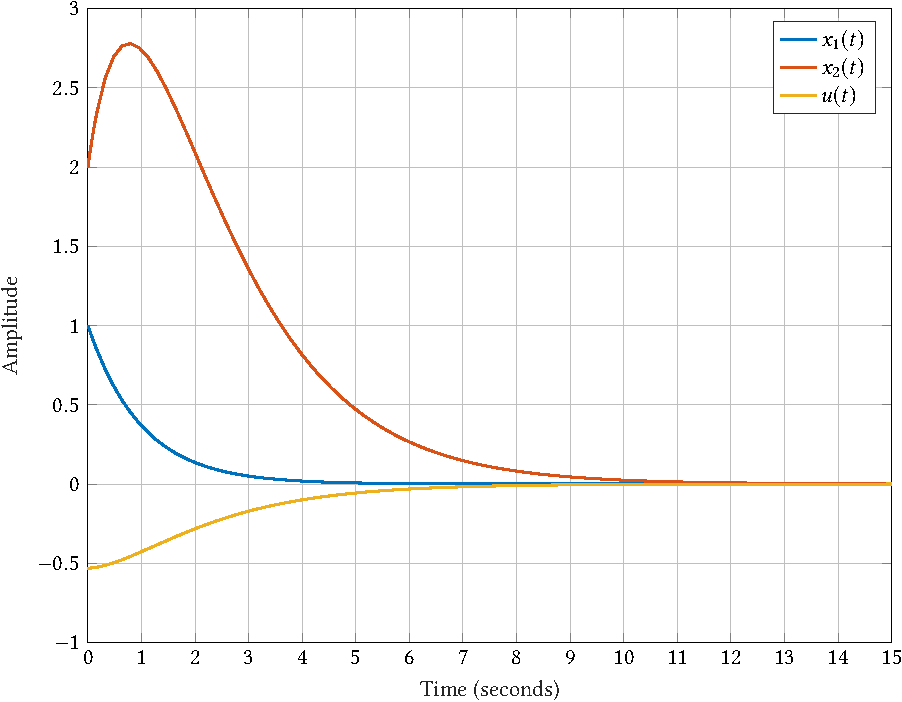
\includegraphics[width=0.9\textwidth]{figures/gcc_linear_bound2.pdf}
    \captionG{Σύστημα με αβεβαιότητες, \( r_1 = 1, r_2 = 1 \)}
    \label{fig:gcc_linear_bound2}
\end{figure}
\begin{figure}[h]
    \centering
    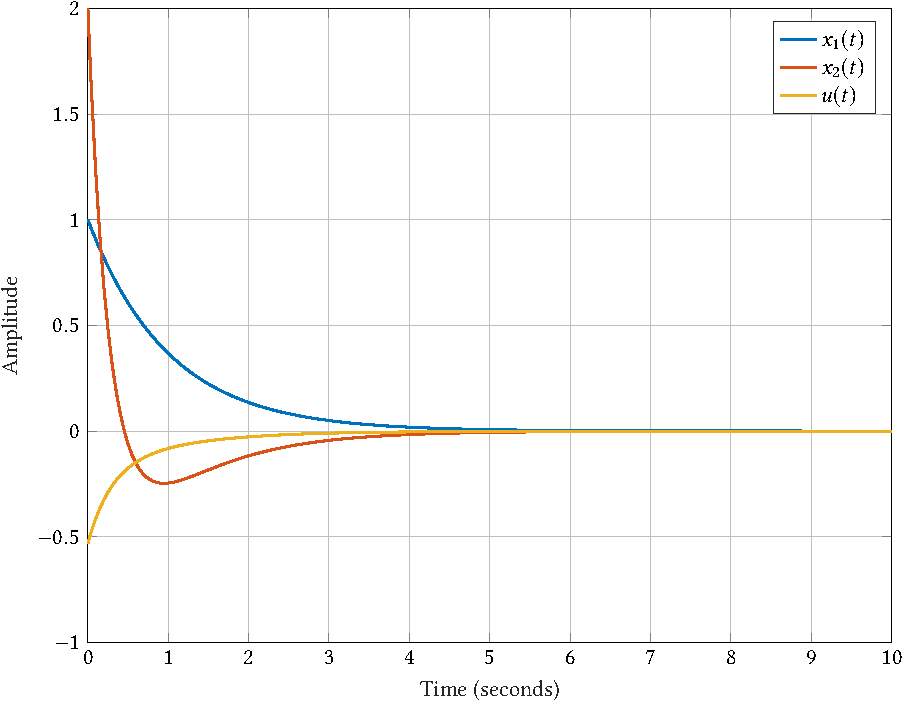
\includegraphics[width=0.9\textwidth]{figures/gcc_linear_bound3.pdf}
    \captionG{Σύστημα με αβεβαιότητες, \( r_1 = -1, r_2 = -1 \)}
    \label{fig:gcc_linear_bound3}
\end{figure}

Στο ίδιο αρχείο κώδικα, γίνεται υλοποίηση του θεωρήματος \( 3.4 \) του
βιβλίου~\cite{kosmidou2009robust}. Σύμφωνα με το θεώρημα αυτό, αν υπάρχει μία
θετικά ορισμένη λύση της γενικευμένης αλγεβρικής εξίσωσης \tl{Riccati} τότε αυτή
μπορεί να βρεθεί επαναληπτικά, επιλύοντας μία εξίσωση \tl{Lyapunov}. Στο
παράδειγμα υλοποιήσαμε το θεώρημα με τη συνάρτηση \mono{gcc\_lyap}. Σαν
αρχική λύση της εξίσωσης \tl{Lyapunov}, όπως αυτή ορίζεται στο αντίστοιχο
θεώρημα, δώσαμε τη λύση που υπολογίσαμε από την πρώτη \mono{fsolve}.
Παρατηρούμε ότι η εξίσωση \tl{Lyapunov} ικανοποιείται για τον πίνακα \( P \)
που υπολογίσαμε και έτσι επιβεβαιώνεται ότι η λύση που υπολογίσαμε είναι όντως η
ζητούμενη.

Ο κώδικας για το παράδειγμα της μεθόδου εγγυημένου κόστους με γραμμικό φράγμα
και αβεβαιότητες στον πίνακα των καταστάσεων παρατίθεται παρακάτω.
\eng{\lstinputlisting[language=Matlab]{src/gcc_linear_bound.m}}

Στο παραπάνω παράδειγμα που παρουσιάσαμε επιλέξαμε την παράμετρο
\( \varepsilon = 1 \).  Όπως αναφέραμε, μέσω της παραμέτρου αυτής
μπορούμε να ικανοποιήσουμε περαιτέρω προδιαγραφές σχεδίασης. Όμως η σχέση του άνω
φράγματος~\eqref{eq:gcc_u_linear}, δεν εξαρτάται γραμμικά από την παράμετρο \(
\varepsilon \) και σίγουρα δεν είναι τετριμμένο το πως επηρεάζει τη λύση της
\tl{GARE}~\eqref{eq:un_gare_general}. Για το λόγο αυτό υλοποιήθηκε πρόγραμμα στο
\tl{MATLAB} όπου ελέγχει την ύπαρξη θετικά ορισμένου πίνακα \( P \) της
\tl{GARE} για το γραμμικό φράγμα, σχέση~\eqref{eq:un_gare_linear},
για τις διάφορες τιμές του \( \varepsilon \).

Τελικά, εκτελώντας τον αντίστοιχο κώδικα βρίσκουμε ότι για τις τιμές της παραμέτρου
\( \varepsilon = (0.7, 0.8, 0.9, 1.0) \) υπάρχει θετικά ορισμένος πίνακας \( P
\) της \tl{GARE}, σχέση~\eqref{eq:un_gare_linear}, και επομένως για τις
κανονικοποιημένες αποδεκτές αβεβαιότητες το κλειστό σύστημα του συγκεκριμένου
παραδείγματος είναι ευσταθές.

Ο κώδικας για το παράδειγμα της μεθόδου εγγυημένου κόστους με γραμμικό φράγμα
και αβεβαιότητες στον πίνακα των καταστάσεων για τις διάφορες τιμές τις
παραμέτρου \( \varepsilon \) παρατίθεται παρακάτω.
\eng{\lstinputlisting[language=Matlab]{src/gcc_linear_bound_all.m}}

Με τον κώδικα που παρουσιάσαμε παραπάνω, είναι πολύ εύκολο προσθέτοντας δύο
βρόχους (\tl{for loops}), κάποιος βρει τις θετικά ορισμένες λύσεις \( P \) της
\tl{GARE} συναρτήσει των μεταβολών των αβεβαιοτήτων \( A_1(r_1), A_2(r_2) \).
Η μετατροπή αυτή είναι τετριμμένη και για αυτό απλά την αναφέρουμε χωρίς να
παραθέσουμε τον αντίστοιχο κώδικα.

\section{Συστήματα με αβεβαιότητα στον πίνακα κατάστασης και στον πίνακα εισόδου}
Θα μελετήσουμε την περίπτωση όπου έχουμε αβεβαιότητες στον πίνακα κατάστασης
αλλά και στον πίνακα εισόδου, δηλαδή ισχύει \( \Delta A \neq 0 \) και \( \Delta
B \neq 0 \). Τότε διακρίνουμε δύο περιπτώσεις φράγματος,
\begin{enumerate}[label = (\enumgreek*)]
    \item αβεβαιότητες που ικανοποιούν τις συνθήκες προσαρμογής,
    \item γενική περίπτωση.
\end{enumerate}

\subsection{Αβεβαιότητες που ικανοποιούν τις συνθήκες προσαρμογής}
Σύμφωνα με τη δημοσίευση~\cite{barmish1983}, αν υποθέσουμε ότι οι αβεβαιότητες
ικανοποιούν τις συνθήκες προσαρμογής, δηλαδή
\[
    \Delta A = \sum_{i = 1}^k B\tilde{A}_ir_i, \quad
    \Delta B = \sum_{i = 1}^l B\tilde{B}_ip_i,
\]
όπου \( B \) είναι ο πίνακας εισόδου και \( \tilde{A}_i, \tilde{B}_i \) είναι
σταθεροί πίνακες κατάλληλων διαστάσεων. Η υπόθεση αυτή δεν είναι ιδιαίτερα
ισχυρή. Εύκολα αποδεικνύεται ότι εφόσον μπορεί οι πίνακες \( A, B \) να γραφτούν
σε κανονική μορφή φάσης τότε οι αβεβαιότητες μπορούν σε γραφτούν σε μορφή που
ικανοποιούν τις συνθήκες προσαρμογής. Στη συνέχεια ορίζουμε
\[
    \Theta_i = a_i^{-2}I_m, \quad
    \Xi_i = a_i^2\tilde{A}^T_i\tilde{A}_i,
\]
με \( i = 1, \dots, k \) και
\[
    \Phi_i = b_i^{-2}I_m,\quad
    \Psi_i = b_i^2R^{-1}\tilde{B}_i^T\tilde{B}_iR^{-1},
\]
με \( i = 1, \dots, l \), όπου \( a_i, b_i \) αυθαίρετες θετικές ποσότητες που
ικανοποιούν περαιτέρω προδιαγραφές σχεδίασης. Τότε η
\[
    \mathcal{U}(P) = \sum_{i = 1}^k\left( \Xi_i + PB\Theta_iB^TP \right)
    + \sum_{i = 1}^l\left[ PB\left( \Phi_i + \Psi_i\right)B^TP \right],
\]
είναι μία συνάρτηση άνω φράγματος. Το πλεονέκτημα που μας δίνει η παραπάνω
έκφραση είναι ότι η \tl{GARE}, σχέση~\eqref{eq:un_gare_general}, μπορεί να
γραφτεί στη μορφή μίας κανονικής αλγεβρικής εξίσωσης \tl{Riccati}
\begin{equation}\label{eq:gcc_quad_ric}
    PA + A^TP - PB\hat{R}^{-1}B^TP + \hat{Q} = 0,
\end{equation}
όπου
\begin{equation}\label{eq:gcc_quad}
    \hat{Q} = Q + \sum_{i = 1}^k\Xi_i, \quad
    \hat{R}^{-1} = R^{-1} - \sum_{i = 1}^k\Theta_i +
    \sum_{i = 1}^l\left( \Phi_i + \Psi_i \right).
\end{equation}
Το πρόβλημα συνεπώς εκπίπτει σε πρόβλημα γραμμικού τετραγωνικού ρυθμιστή και
έχει μοναδική θετικά ορισμένη λύση \( P \), όταν το πίνακας \( \hat{R} \) είναι
θετικά ορισμένος.

Θα εφαρμόσουμε τα παραπάνω σε ένα παράδειγμα. Θα θεωρήσουμε το σύστημα που
είδαμε προηγουμένως, δηλαδή
\[
    \dot{x} = Ax + Bu,
\]
όπου οι πίνακες \( A \) και \( B \) είναι
\[
    A =
    \begin{bmatrix}
        -1 & 0 \\
        1 & -2
    \end{bmatrix}, \quad
    B = \begin{bmatrix}0 \\ 1\end{bmatrix}.
\]
Τα μητρώα στάθμισης του δείκτη απόδοσης, σχέση~\eqref{eq:un_cost}, επιλέχθηκαν
\( Q = I_3 \) και \( R = 10 \). Σε αντίθεση με το προηγούμενο παράδειγμα θα
επιλέξουμε πιο ακραίες αβεβαιότητες. Συνεπώς, επιλέξαμε για τον πίνακα
κατάστασης
\[
    \tilde{A}_1 = \begin{bmatrix}5.5 & 0\end{bmatrix},\quad
    \tilde{A}_2 = \begin{bmatrix}0 & 2\end{bmatrix},
\]
όπου σύμφωνα με τους συμβολισμούς έχουμε \( k = 2 \) και για τον πίνακα ελέγχου
\[
    \tilde{B} = 2.5,
\]
όπου έχουμε \( l = 1 \). Άρα οι αβεβαιότητες είναι
\[
    \Delta A(r_1, r_2) =
    B\left(\tilde{A}_1r_1 + \tilde{A}_2r_2\right), \quad
    \Delta B(p_1) = B\tilde{B}_1p_1.
\]
Χωρίς μείωση της γενικότητας βρούμε τον εγγυημένο νόμο ελέγχου για τις
κανονικοποιημένες αποδεκτές αβεβαιότητες, δηλαδή \( |r_1| \leq 1, |r_2| \leq 1
\) και \( |p_1| \leq 1 \). Σαν πρώτη θεώρηση θα επιλέξουμε τις βαθμωτές σταθερές
ίσες με \( a_1 = a_2 = 1 \) και \( b_1 = 1 \), και στη συνέχεια κάποιος μπορεί
μέσω των ποσοτήτων αυτών να βελτιστοποιήσει ως προς κάποια έννοια τα αποτελέσματα μας.
Τελικά, πραγματοποιώντας τους υπολογισμούς βρίσκουμε
\[
    \Theta = \sum_{i = 1}^l\Theta_i = 2, \quad
    \Xi = \sum_{i = 1}^l\Xi_i =
    \begin{bmatrix}
        30.25 & 0 \\
         0 & 4
     \end{bmatrix}
\]
και
\[
    \Phi = \sum_{i = 1}^l\Phi_i = 2,\quad
    \Psi = \sum_{i = 1}^l\Psi_i = 0.0625.
\]
Ακόμα από τις σχέσεις~\eqref{eq:gcc_quad} προκύπτει
\[
    \hat{Q} =
    \begin{bmatrix}
        31.25 & 0 \\
         0 & 5
     \end{bmatrix}, \quad
     \hat{R}^{-1} = 0.1625.
\]
Ο θετικά ορισμένος πίνακας \( P \) της γενικευμένης αλγεβρικής εξίσωσης
\tl{Riccati} μπορεί να βρεθεί με την εντολή \mono{care} του \tl{MATLAB},
με ορίσματα τους πίνακες \( (A, B, \hat{Q}, \hat{R} ) \). Έτσι βρίσκουμε ότι ο
πίνακας \( P \) είναι
\[
  P =
  \begin{bmatrix}
      15.987 & 0.3733 \\
      0.3733 & 1.1923
  \end{bmatrix}.
\]
Όπως παρατηρούμε ο πίνακας είναι συμμετρικός και θετικά ορισμένος, με ιδιοτιμές
\( \lambda_{1,2} = 1.1828, 15.9964 \). Εφόσον η σχέση~\eqref{eq:gcc_quad_ric}
είναι της μορφής του γραμμικού τετραγωνικού ρυθμιστή \tl{LQR}, ως γνωστόν ο
νόμος ελέγχου εγγυημένου κόστους υπολογίζεται
\[
    \tilde{u}(t) = - \hat{R}^{-1}B^{T}Px(t) =
    \begin{bmatrix}
        -0.0607 & -0.193
    \end{bmatrix}x(t).
\]
Το εγγυημένο κόστος υπολογίζεται από τη σχέση~\eqref{eq:un_gcc_J}
\[
   \tilde{J} = \tr{P} = 17.1792
\]
ενώ από τη σχέση που εξαρτάται από τις αρχικές συνθήκες
\[
    \tilde{J}(x_0) = x_0^{T}Px_0 =
    \begin{bmatrix}
        -1 & 2
    \end{bmatrix}P
    \begin{bmatrix}
        -1 & 2
    \end{bmatrix}^T = 19.2628.
\]
Στα σχήματα~\ref{fig:gcc_quad_bound1},~\ref{fig:gcc_quad_bound2}
και~\ref{fig:gcc_quad_bound3} παρουσιάζονται οι καταστάσεις του συστήματος για
τις διάφορες τιμές των αβεβαιοτήτων καθώς και ο νόμος ελέγχου εγγυημένου
κόστους.
\begin{figure}[h]
    \centering
    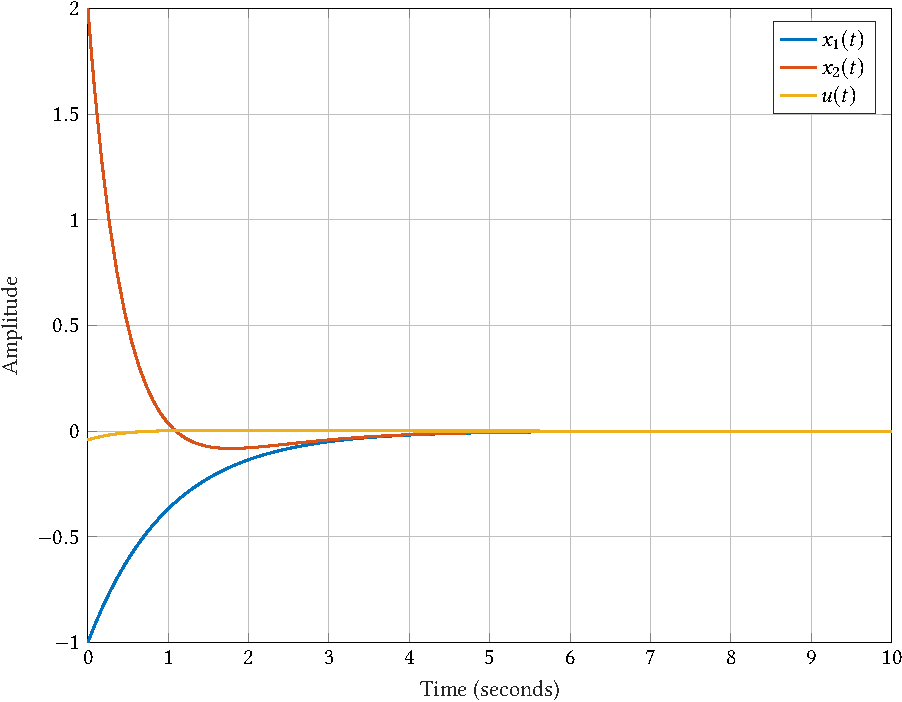
\includegraphics[width=0.9\textwidth]{figures/gcc_quad_bound1.pdf}
    \captionG{Αρχικό σύστημα χωρίς αβεβαιότητες}
    \label{fig:gcc_quad_bound1}
\end{figure}
\begin{figure}[h]
    \centering
    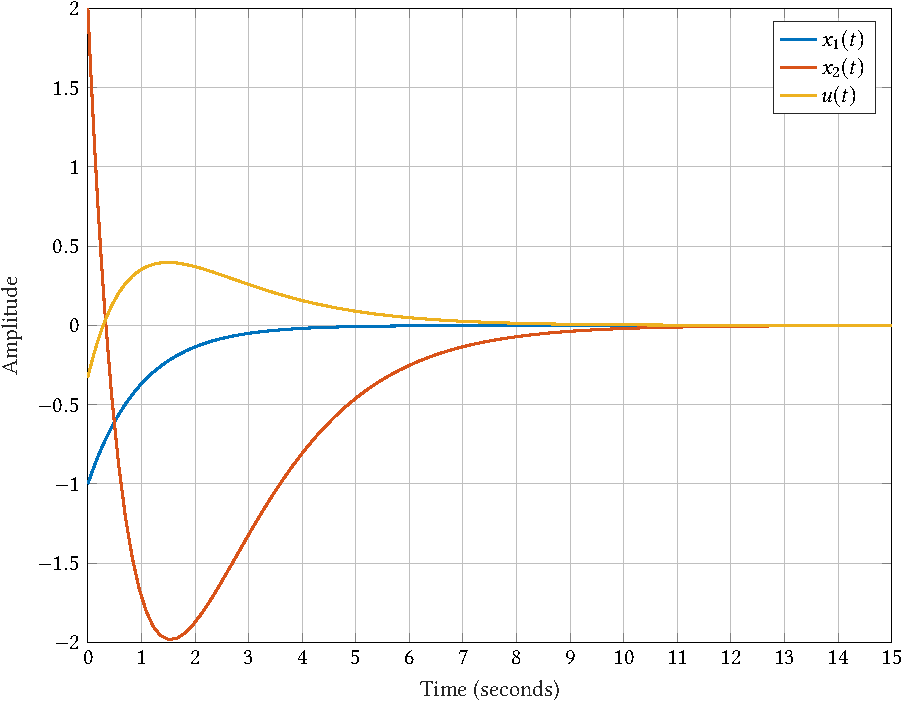
\includegraphics[width=0.9\textwidth]{figures/gcc_quad_bound2.pdf}
    \captionG{Σύστημα με αβεβαιότητες, \( r_1 = 1, r_2 = 1, p_1 = 1 \)}
    \label{fig:gcc_quad_bound2}
\end{figure}
\begin{figure}[h]
    \centering
    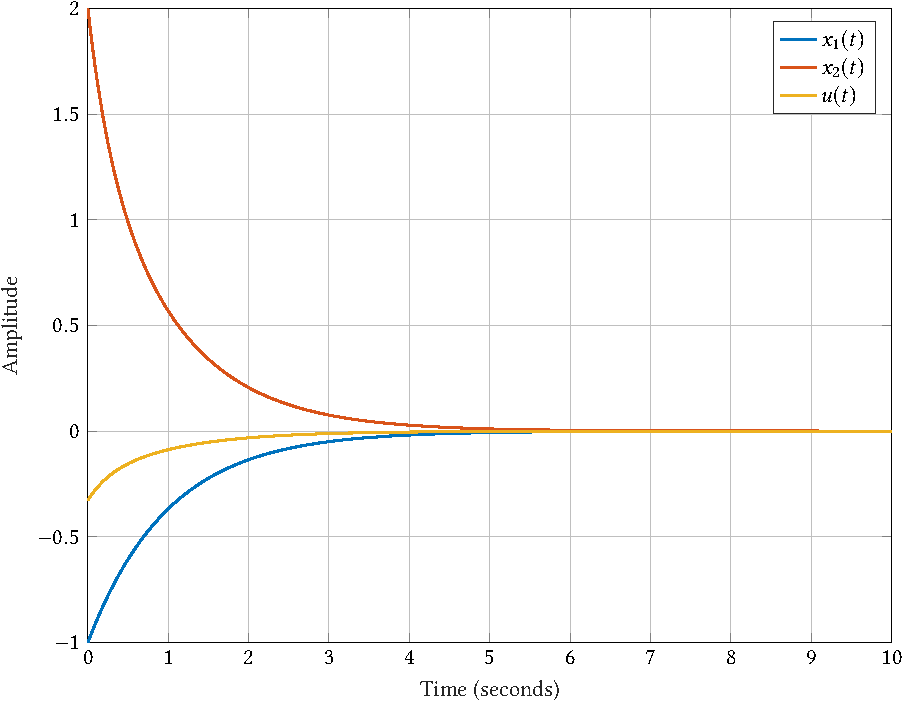
\includegraphics[width=0.9\textwidth]{figures/gcc_quad_bound3.pdf}
    \captionG{Σύστημα με αβεβαιότητες, \( r_1 = -1, r_2 = -1, p_1 = -0.5 \)}
    \label{fig:gcc_quad_bound3}
\end{figure}

Ο κώδικας για το παράδειγμα της μεθόδου εγγυημένου κόστους με τετραγωνικό φράγμα
και αβεβαιότητες στον πίνακα των καταστάσεων αλλά και ελέγχου παρατίθεται παρακάτω.
\eng{\lstinputlisting[language=Matlab]{src/gcc_quad_bound.m}}

\subsection{Γενική περίπτωση}
Στην περίπτωση αυτή οι αβεβαιότητες μπορούν να γραφτούν στη μορφή
\[
    A_i = d_ie_i^T, \quad
    B_j = f_jg_j^T,
\]
όπου \( i = 1, \dots, k \) και \( j = 1, \dots, l \) και \(d_i, e_i, f_j, g_j \)
διανύσματα κατάλληλων διαστάσεων. Είναι προφανές ότι η επιλογή των διανυσμάτων
δεν είναι μοναδική. Στη συνέχεια ορίζονται οι συμμετρικοί και θετικά ορισμένοι
πίνακες
\[
    T = \sum_{i = 1}^k d_id_i^T, \quad
    U = \sum_{i = 1}^k e_ie_i^T,
\]
και
\[
    V = \sum_{i = 1}^l g_ig_i^T, \quad
    W = \sum_{i = 1}^l f_if_i^T.
\]
Αποδεικνύεται ότι η παρακάτω έκφραση
\[
    \mathcal{U}(P) = PTP + U + PWP + PBR^{-1}VR^{-1}B^TP
\]
αποτελεί συνάρτηση άνω φράγματος της \eqref{eq:un_bound}. Η γενικευμένη αλγεβρική εξίσωση
\tl{Riccati} γίνεται επομένως
\begin{equation}\label{eq:gcc_quad_gen_gare}
    PA + A^TP - P
    \left(\varepsilon^{-1}BR^{-1}B^T - \varepsilon^{-2}BR^{-1}VR^{-1}B - W - T\right)
    P + Q + \mathcal{U}(P) = 0.
\end{equation}
Η παραπάνω είναι μη γραμμική αλγεβρική εξίσωση ως προς \( P \). Δεν έχουμε
γενική αναλυτική λύση αλλά ούτε και συνθήκες ύπαρξης λύσης. Στόχος είναι η
εύρεση θετικά ορισμένου συμμετρικού πίνακα \( P \). Η επίλυση της υλοποιήθηκε
με τη μέθοδο \tl{Newton-Raphson}, όπως και στην περίπτωση του γραμμικού φράγματος.
Τα τεχνικά της μεθόδου αναφέρονται παραπάνω και δεν θα τα επαναλάβουμε,
καθώς η διαδικασία είναι όμοια. Ακόμα προσθέσαμε την παράμετρο
\( \varepsilon \in (0, 1] \) ούτως ώστε να ικανοποιήσουμε περαιτέρω κριτήρια
σχεδιασμού. Συνεπώς, ο νόμος ελέγχου εγγυημένου κόστους, όπως και προηγουμένως είναι
\begin{equation}\label{eq:gcc_quad_gen_u}
    u(t) = -\varepsilon^{-1}R^{-1}B^{T}Px(t).
\end{equation}
Αποδεικνύεται ότι η ικανή και αναγκαία συνθήκη ώστε η \tl{GARE} να έχει λύση,
δηλαδή να βρούμε θετικά ορισμένο συμμετρικό πίνακα \( P \), είναι αν και μόνο
αν ο πίνακας \( H \),
\[
    H =
    \begin{bmatrix}
        A & -M(\varepsilon) \\
        -Q - U & -A^T
    \end{bmatrix},
\]
όπου
\[
    M(\varepsilon) =
    \varepsilon^{-1}BR^{-1}B^T - \varepsilon^{-2}BR^{-1}VR^{-1}B - W - T,
\]
δεν έχει καθαρά φανταστικές ιδιοτιμές. Παρόλο αυτά, αξίζει να σημειωθεί ότι
η \tl{GARE}, σχέση~\eqref{eq:gcc_quad_gen_gare}, λόγω της μη γραμμικότητας
μπορεί να έχει λύσεις με \( P \) όχι συμμετρικό που σταθεροποιούν το κλειστό
σύστημα.

Όπως και στις προηγούμενες μεθόδους, θα παρουσιάσουμε ένα παράδειγμα. Αυτή τη
φορά θα διαφοροποιήσουμε το σύστημα. Θα θεωρήσουμε το σύστημα
\[
    \dot{x} = Ax + Bu,
\]
όπου οι πίνακες \( A \) και \( B \) είναι
\[
    A =
    \begin{bmatrix}
        -1 & 2 \\
        -1 & -1
    \end{bmatrix}, \quad
    B = \begin{bmatrix}0 \\ 1\end{bmatrix}.
\]
Τα μητρώα στάθμισης του δείκτη απόδοσης, σχέση~\eqref{eq:un_cost}, επιλέχθηκαν
\( Q = I_3 \) και \( R = 10 \). Οι αβεβαιότητες για τον πίνακα κατάστασης
επιλέχθηκαν
\[
    A_1 =
    \begin{bmatrix}
        0.54 & 0.18 \\
        0.18 &  0.06
    \end{bmatrix},\quad
    A_2 =
    \begin{bmatrix}
        0.04 & 0.09 \\
        0.12 & 0.27
    \end{bmatrix},
\]
που οδηγεί
\[
    \Delta A(r_1, r_2) = r_1A_1 + r_2A_2,
\]
και για τον πίνακα ελέγχου έχουμε
\[
    B_1 =
    \begin{bmatrix}
        0.18 \\
        0.12
    \end{bmatrix}
\]
και άρα
\[
    \Delta B(p_1) = p_1B_1.
\]
Οι αβεβαιότητες συνεπώς μπορούν να γραφτούν
\[
    d_1 =
    \begin{bmatrix}
        0.9 \\ 0.3
    \end{bmatrix},\quad
    e_1 =
    \begin{bmatrix}
        0.6 \\ 0.2
    \end{bmatrix},\quad
    d_2 =
    \begin{bmatrix}
        0.1 \\ 0.3
    \end{bmatrix},\quad
    e_2 =
    \begin{bmatrix}
        0.4 \\ 0.9
    \end{bmatrix}
    f_1 =
    \begin{bmatrix}
        0.3 \\ 0.2
    \end{bmatrix},\quad
    g_1 = 0.6.
\]
Ακόμα σύμφωνα με τα παραπάνω ορίζονται οι συμμετρικοί και θετικά ορισμένοι
πίνακες
\[
    T =
    \begin{bmatrix}
        0.82 & 0.3 \\
        0.3 & 0.18
    \end{bmatrix},\quad
    U =
    \begin{bmatrix}
        0.52 & 0.48 \\
        0.48 & 0.85
    \end{bmatrix},
\]
και
\[
    V = 0.36,\quad
    W =
    \begin{bmatrix}
        0.09 & 0.06 \\
        0.06 & 0.04
    \end{bmatrix}.
\]
Στο παράδειγμα επιλέξαμε την παράμετρο \( \varepsilon = 1 \) και δίχως μείωση της
γενικότητας βρήκαμε το εγγυημένο κόστος για τα κανονικοποιημένα όρια των αποδεκτών
αβεβαιοτήτων, δηλαδή για
\( |r_1| \leq 1 , |r_2| \leq 1 \) και \( |p_1| \leq 1 \). Στη συνέχεια κάποιος
μπορεί να λύσει την \tl{GARE}~\eqref{eq:gcc_quad_gen_gare}, για τις διάφορες
τιμές του \( \varepsilon \), όπως κάναμε στην περίπτωση του γραμμικού φράγματος.

Ο θετικά ορισμένος πίνακας \( P \) της γενικευμένης αλγεβρικής εξίσωσης
\tl{Riccati} υπολογίσθηκε με την εντολή \mono{fsolve} του \tl{MATLAB}, υλοποιεί
τη μέθοδο \tl{Newton-Raphson}. Έτσι βρίσκουμε ότι ο πίνακας \( P \) είναι
\[
    P =
    \begin{bmatrix}
        0.7806 & 0.3686 \\
        0.3686 & 2.3976
    \end{bmatrix}.
\]
Όπως παρατηρούμε ο πίνακας είναι συμμετρικός και θετικά ορισμένος, με ιδιοτιμές
\( \lambda_{1,2} = 0.7005, 2.4777 \). Ακόμα από τη σχέση~\eqref{eq:gcc_quad_gen_u}
ο νόμος ελέγχου εγγυημένου κόστους υπολογίζεται
\[
    \tilde{u}(t) =
    \begin{bmatrix}
        -0.0369 & -0.2398
    \end{bmatrix}x(t).
\]
Το εγγυημένο κόστος υπολογίζεται από τη σχέση~\eqref{eq:un_gcc_J}
\[
   \tilde{J} = \tr{P} = 3.1781
\]
ενώ από τη σχέση που εξαρτάται από τις αρχικές συνθήκες
\[
    \tilde{J}(x_0) = x_0^{T}Px_0 =
    \begin{bmatrix}
        3 & -2
    \end{bmatrix}P
    \begin{bmatrix}
        3 & -2
    \end{bmatrix}^T = 12.1916.
\]
Ακόμη οι ιδιοτιμές του πίνακα \( H \) δεν είναι καθαρά φανταστικές και επομένως
ικανοποιείται η συνθήκη της ικανής και αναγκαίας συνθήκης για την ύπαρξη λύσης,
κάτι που επιβεβαιώνει τους υπολογισμούς που πραγματοποιήθηκαν.

Στα σχήματα~\ref{fig:gcc_quad_bound_gen1},~\ref{fig:gcc_quad_bound_gen2}
και~\ref{fig:gcc_quad_bound_gen3} παρουσιάζονται οι καταστάσεις του συστήματος για
τις διάφορες τιμές των αβεβαιοτήτων καθώς και ο νόμος ελέγχου εγγυημένου
κόστους.
\begin{figure}[h]
    \centering
    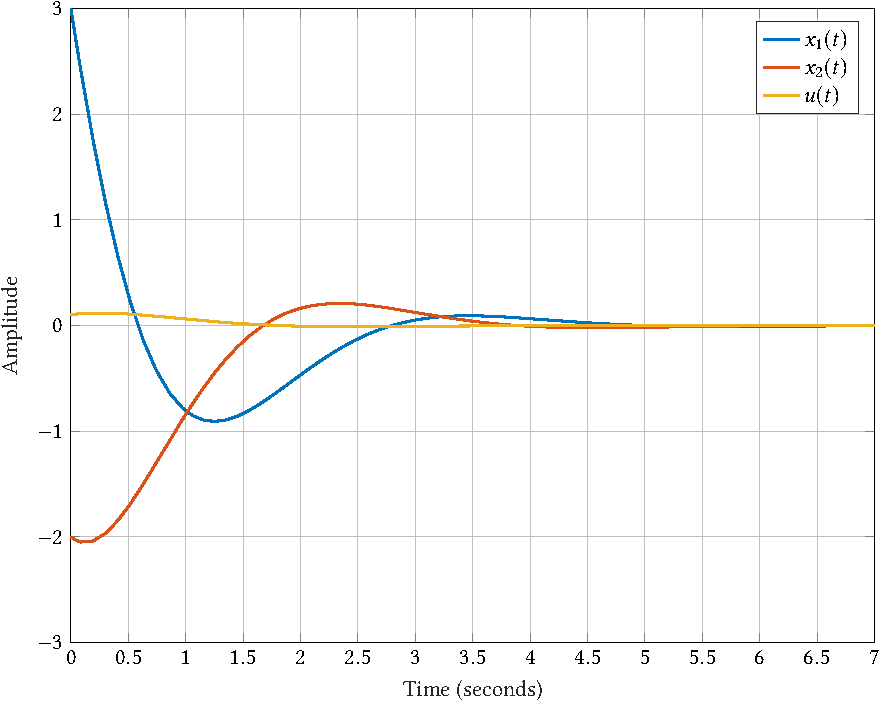
\includegraphics[width=0.9\textwidth]{figures/gcc_quad_bound_gen1.pdf}
    \captionG{Αρχικό σύστημα χωρίς αβεβαιότητες}
    \label{fig:gcc_quad_bound_gen1}
\end{figure}
\begin{figure}[h]
    \centering
    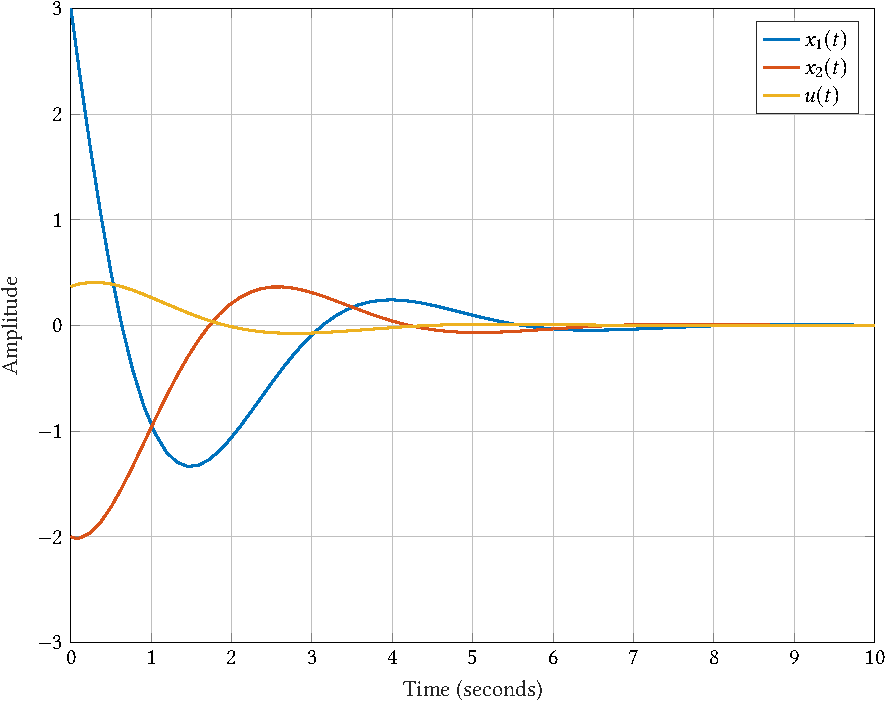
\includegraphics[width=0.9\textwidth]{figures/gcc_quad_bound_gen2.pdf}
    \captionG{Σύστημα με αβεβαιότητες, \( r_1 = 1, r_2 = 1, p_1 = 1 \)}
    \label{fig:gcc_quad_bound_gen2}
\end{figure}
\begin{figure}[h]
    \centering
    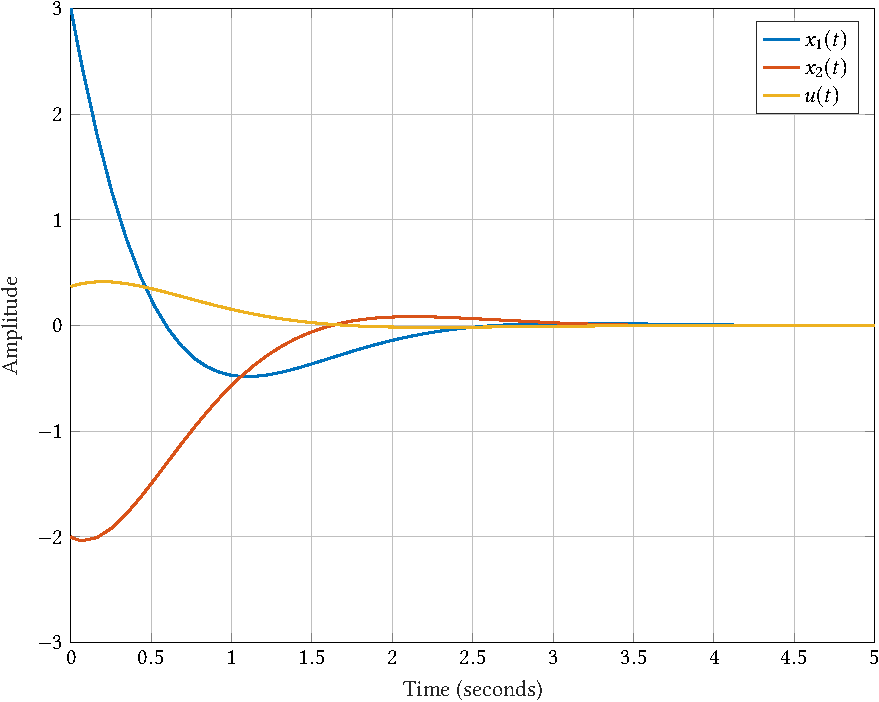
\includegraphics[width=0.9\textwidth]{figures/gcc_quad_bound_gen3.pdf}
    \captionG{Σύστημα με αβεβαιότητες, \( r_1 = -1, r_2 = -1, p_1 = -1 \)}
    \label{fig:gcc_quad_bound_gen3}
\end{figure}

Ο κώδικας για το παράδειγμα της μεθόδου εγγυημένου κόστους για τη γενική
περίπτωση με αβεβαιότητες στον πίνακα των καταστάσεων και πίνακα ελέγχου
παρατίθεται παρακάτω.
\eng{\lstinputlisting[language=Matlab]{src/gcc_quad_bound_gen.m}}

\section{Ελαχιστοποίηση του εγγυημένου κόστους}
Η προσέγγιση μέχρι τώρα της επίλυσης των γενικευμένων αλγεβρικών εξισώσεων
\tl{Riccati} οδηγεί σε υψηλές τιμές του εγγυημένου κόστους. Αυτό διότι το
εγγυημένο κόστος είναι ανάλογο της λύσης \( P \) της \tl{GARE}. Επομένως θα
μπορούσαμε να εκφράσουμε το πρόβλημα ως ένα πρόβλημα ελαχιστοποίησης του
εγγυημένου κόστους, ή ισοδύναμα του ίχνους του \( P \),
σχέση~\eqref{eq:un_gcc_J}. Η κατάστρωση ενός τέτοιου προβλήματος ελαχιστοποίησης
είναι μία δύσκολη διαδικασία και γίνεται ακόμα δυσκολότερη καθώς αυξάνονται οι
διαστάσεις του προβλήματος. Όμως αν διατυπώσουμε το πρόβλημα ως ένα πρόβλημα
κυρτής βελτιστοποίησης, μέσω των γραμμικών ανισοτήτων πινάκων
\tl{LMI} τότε μπορούμε με ευκολία να καταστρώσουμε και να επιλύσουμε το εν λόγω
πρόβλημα.

Οι αβεβαιότητες μπορούν να γραφτούν στη μορφή
\[
    A_i = \sigma_i^{1/2}d_i\sigma_i^{-1/2}e_i^T, \quad
    B_j = \tau_i^{1/2}f_j\tau_i^{-1/2}g_j^T,
\]
όπου \( i = 1, \dots, k \) και \( j = 1, \dots, l \) και \(d_i, e_i, f_j, g_j \)
διανύσματα κατάλληλων διαστάσεων και \( \sigma_i, \tau_i \) είναι θετικές
βαθμωτές ποσότητες. Στην προηγούμενη μέθοδο είχαμε επισημάνει ότι η επιλογή των
διανυσμάτων δεν είναι μοναδική. Έτσι μπορούμε να θεωρήσουμε ως μεταβλητές του
προβλήματος ελαχιστοποίησης τις ποσότητες \( \sigma_i, \tau_i \). Στη συνέχεια
ορίζονται οι πίνακες
\[
    D = \begin{bmatrix} d_1 & \dots & d_k\end{bmatrix}, \quad
    E = \begin{bmatrix} e_1 & \dots & e_k\end{bmatrix}^T,
\]
και
\[
    F = \begin{bmatrix} f_1 & \dots & f_l\end{bmatrix}, \quad
    G = \begin{bmatrix} g_1 & \dots & g_l\end{bmatrix}.
\]
Ακόμα ορίζονται οι διαγώνιοι πίνακες
\[
    \tilde{S} = \diag\begin{pmatrix} \sigma_1 & \dots & \sigma_k\end{pmatrix}, \quad
    \tilde{T} = \diag\begin{pmatrix} \tau_1 & \dots & \tau_l\end{pmatrix}.
\]
Η \tl{GARE}~\eqref{eq:gcc_quad_gen_gare} έχει μία θετικά ορισμένη λύση
τέτοια ώστε το αντίστοιχο εγγυημένο κόστος να γίνεται ελάχιστο, αν
ισχύει το πρόβλημα ελαχιστοποίησης που διατυπώνεται στο παρακάτω θεώρημα.

\begin{theorem}[Θεώρημα 3.5 της Κοσμίδου~\cite{kosmidou2009robust}]
    Έστω το αβέβαιο σύστημα~\eqref{eq:un_ss} και το αντίστοιχο τετραγωνικό
    κριτήριο~\eqref{eq:un_cost}. Αν υπάρχουν συμμετρικοί και θετικά ορισμένοι
    πίνακες \( \tilde{M}, \tilde{P} \), διαγώνιοι και θετικά ορισμένοι πίνακες
    \( \tilde{S}, \tilde{T} \) και ένας θετικός αριθμός \( \delta \), τέτοιοι
    ώστε το ακόλουθο πρόβλημα ελαχιστοποίησης
    \begin{equation*}
        \begin{aligned}
            & \underset{
                (\tilde{M}, \tilde{P}, \tilde{S}, \tilde{T}, \delta)
            }{\mathtxt{minimize}}
            & & \tr \tilde{M} \\
            & \mathtxt{subject to}
            & &
            \begin{bmatrix}
                \tilde{M} & I \\
                I & \tilde{P}
            \end{bmatrix} > 0 \\
            &&&
            \begin{bmatrix}
                -\tilde{P}A^T - A\tilde{P} + \delta BR^{-1}B^T
                - D\tilde{S}D^T - F\tilde{T}F^T & \tilde{P}E^T &
                \delta BR^{-1}G^T & \tilde{P} \\
                E\tilde{P} & \tilde{S} & 0 & 0 \\
                \delta GR^{-1}B^T & 0 & \tilde{T} & 0 \\
                \tilde{P} & 0 & 0 & Q_0^{-1}\\
            \end{bmatrix} > 0,
        \end{aligned}
    \end{equation*}
    έχει ένα μη κενό σύνολο εφικτών λύσεων
    \( \left( \tilde{M}, \tilde{P}, \tilde{S}, \tilde{T}, \delta \right) \), τότε
    ο νόμος ελέγχου
    \[
        u^*(t) = -\delta R^{-1}B^TPx(t)
    \]
    είναι ένας νόμος ελέγχου εγγυημένου κόστους και
    \[
        J^* = \tr P
    \]
    είναι το εγγυημένο κόστος για το σύστημα~\eqref{eq:un_ss} με τυχαίες αρχικές
    συνθήκες, όπου \( P = \tilde{P}^{-1} \) και \( \delta = 1/\varepsilon \).
\end{theorem}

Αποδεικνύεται ότι για οποιοδήποτε \( Q_0 < Q \), η επίλυση του \tl{LMI} που
διατυπώνεται στο παραπάνω θεώρημα, ισοδυναμεί με την επίλυση της
\tl{GARE}~\eqref{eq:gcc_quad_gen_gare}. Η μεταβλητή \( \tilde{M} \) είναι μία
εικονική μεταβλητή (\tl{dummy variable}). Από την πρώτη γραμμική ανισότητα
πινάκων, αν πάρουμε το συμπλήρωμα του \tl{Schur} προκύπτει
\[
    \tilde{P} > 0 \quad \text{και}\quad \tilde{M} - \tilde{P}^{-1} > 0,
\]
ή ισοδύναμα
\[
    \tilde{M} - P > 0.
\]
Επομένως ελαχιστοποιώντας τον πίνακα \( \tilde{M} \), ή αντίστοιχα το
\( \tr \tilde{M} \), ελαχιστοποιούμε τον πίνακα \( \tilde{P} \), ή αντίστοιχα το
\( \tr \tilde{P} \) και άρα το εγγυημένο κόστος.

Θα παρουσιάσουμε το παράδειγμα που μελετήσαμε και προηγουμένως για σύγκριση των
αποτελεσμάτων. Για ευκολία παραθέτουμε ξανά το σύστημα
\[
    \dot{x} = Ax + Bu,
\]
όπου οι πίνακες \( A \) και \( B \) είναι
\[
    A =
    \begin{bmatrix}
        -1 & 2 \\
        -1 & -1
    \end{bmatrix}, \quad
    B = \begin{bmatrix}0 \\ 1\end{bmatrix}.
\]
Τα μητρώα στάθμισης του δείκτη απόδοσης, σχέση~\eqref{eq:un_cost}, επιλέχθηκαν
\( Q = I_3 \) και \( R = 10 \). Για το πρόβλημα ελαχιστοποίησης οριακά θεωρούμε
\( Q_0 = Q \). Οι αβεβαιότητες επιλέχθηκαν και διατυπώθηκαν μέσω των πινάκων
\[
    D =
    \begin{bmatrix}
        0.9 & 0.1 \\
        0.3 & 0.3
    \end{bmatrix},\quad
    E =
    \begin{bmatrix}
        0.6 & 0.2 \\
        0.4 & 0.9
    \end{bmatrix},\quad
    F =
    \begin{bmatrix}
        0.3 \\ 0.2
    \end{bmatrix},\quad
    G = 0.6.
\]
Με τον κώδικα στο πρόγραμμα \tl{MATLAB} που παραθέτουμε παρακάτω επιλύσαμε το
πρόβλημα ελαχιστοποίησης με τις γραμμικές ανισότητες πινάκων. Τελικά,
υπολογίζουμε τις μεταβλητές ελαχιστοποίησης στο βέλτιστο σημείο
\[
    \tilde{M} =
    \begin{bmatrix}
        0.7394 & 0.2879 \\
        0.2879 & 1.8596
    \end{bmatrix},\quad
    \tilde{P} =
    \begin{bmatrix}
        1.4391 & -0.2228 \\
        -0.2228 & 0.5722
    \end{bmatrix},
\]
και
\[
    \tilde{S} = \diag
    \begin{pmatrix}
        0.6586 & 1.7735
    \end{pmatrix},\quad
    \tilde{T} = 2.0098e-06, \quad
    \delta = 2.7145e-09.
\]
Από τη σχέση \( P = \tilde{P}^{-1} \) βρίσκουμε
\[
    P =
    \begin{bmatrix}
        0.7394 & 0.2879 \\
        0.2879 & 1.8596
    \end{bmatrix},
\]
που παρατηρούμε ότι είναι συμμετρικός και θετικά ορισμένος και έχει ιδιοτιμές
\( \lambda_{1,2} = 0.6698, 1.9293 \). Ακόμα ο νόμος ελέγχου εγγυημένου κόστους
υπολογίζεται
\begin{align*}
    \tilde{u}^*(t) &=
    -\delta R^{-1} B^T P x(t) \\
    &= 1.0e-09
    \begin{bmatrix}
        -0.0782 & -0.5048
    \end{bmatrix}x(t).
\end{align*}
Το εγγυημένο κόστος υπολογίζεται
\[
    \tilde{J}^* = \tr{P} = 2.5990,
\]
ενώ από τη σχέση που εξαρτάται από τις αρχικές συνθήκες
\[
    \tilde{J}^*(x_0) = x_0^{T}Px_0 =
    \begin{bmatrix}
        3 & -2
    \end{bmatrix}P
    \begin{bmatrix}
        3 & -2
    \end{bmatrix}^T = 10.6383.
\]
Αντίστοιχα το κόστος του αρχικού συστήματος υπολογίζεται
\[
    \tilde{J}^*_{not} = \tr{P}_{not} = 1.0643,
\]
ενώ από τη σχέση που εξαρτάται από τις αρχικές συνθήκες
\[
    \tilde{J}^*_{not}(x_0) = x_0^{T}P_{not}x_0 =
    \begin{bmatrix}
        3 & -2
    \end{bmatrix}P_{not}
    \begin{bmatrix}
        3 & -2
    \end{bmatrix}^T = 5.2966.
\]
Παρατηρούμε ότι ακριβώς το ίδιο πρόβλημα με το προηγούμενο μας δίνει βελτιωμένο,
μικρότερο εγγυημένο κόστος πιο κοντά στο αρχικό κόστος που παρουσιάζει το
σύστημα χωρίς αβεβαιότητες, που είναι φυσικά και το αναμενόμενο αποτέλεσμα.
Ακόμα παρατηρούμε ότι ο νόμος ελέγχου εγγυημένου κόστους είναι ουσιαστικά
μηδενικός. Αυτό είναι λογικό διότι ο συντελεστής \( R \) του \( u(t) \) είναι
υψηλός και εφόσον ο πίνακας \( A \) είναι \tl{Hurwitz}, η μηδενική δράση οδηγεί
σε ελαχιστοποίηση του κόστους.

Στα σχήματα~\ref{fig:gcc_lmi1},~\ref{fig:gcc_lmi2}
και~\ref{fig:gcc_lmi3} παρουσιάζονται οι καταστάσεις του συστήματος για
τις διάφορες τιμές των αβεβαιοτήτων καθώς και ο νόμος ελέγχου εγγυημένου
κόστους.
\begin{figure}[h]
    \centering
    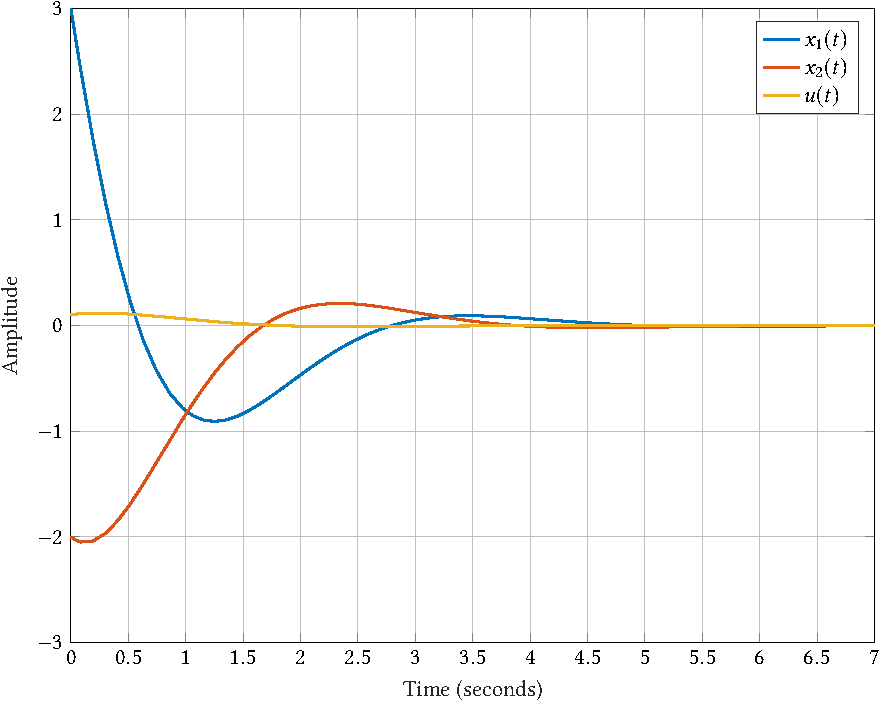
\includegraphics[width=0.9\textwidth]{figures/gcc_lmi1.pdf}
    \captionG{Αρχικό σύστημα χωρίς αβεβαιότητες}
    \label{fig:gcc_lmi1}
\end{figure}
\begin{figure}[h]
    \centering
    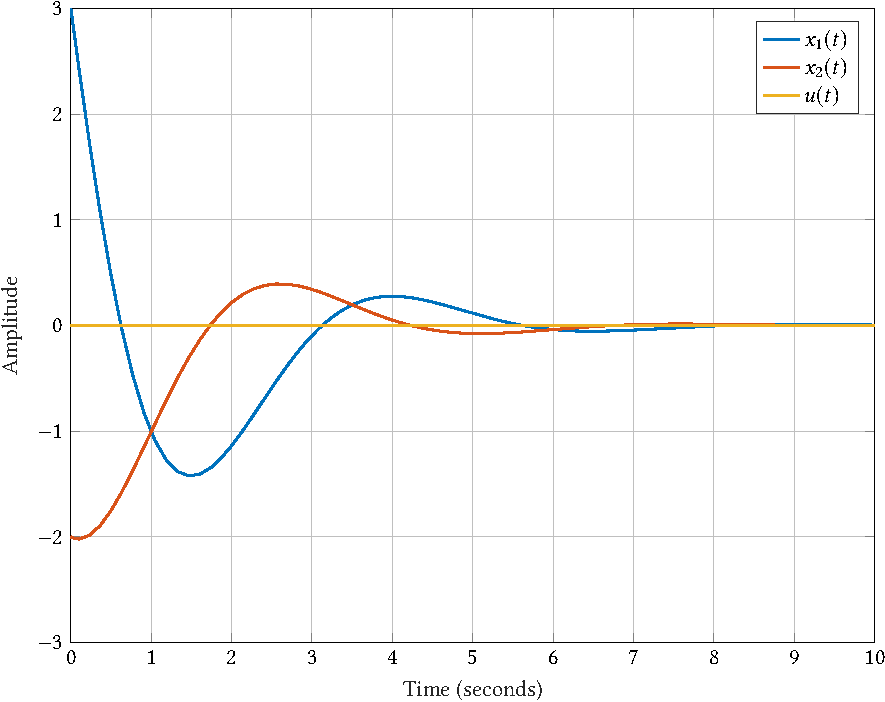
\includegraphics[width=0.9\textwidth]{figures/gcc_lmi2.pdf}
    \captionG{Σύστημα με αβεβαιότητες, \( r_1 = 1, r_2 = 1, p_1 = 1 \)}
    \label{fig:gcc_lmi2}
\end{figure}
\begin{figure}[h]
    \centering
    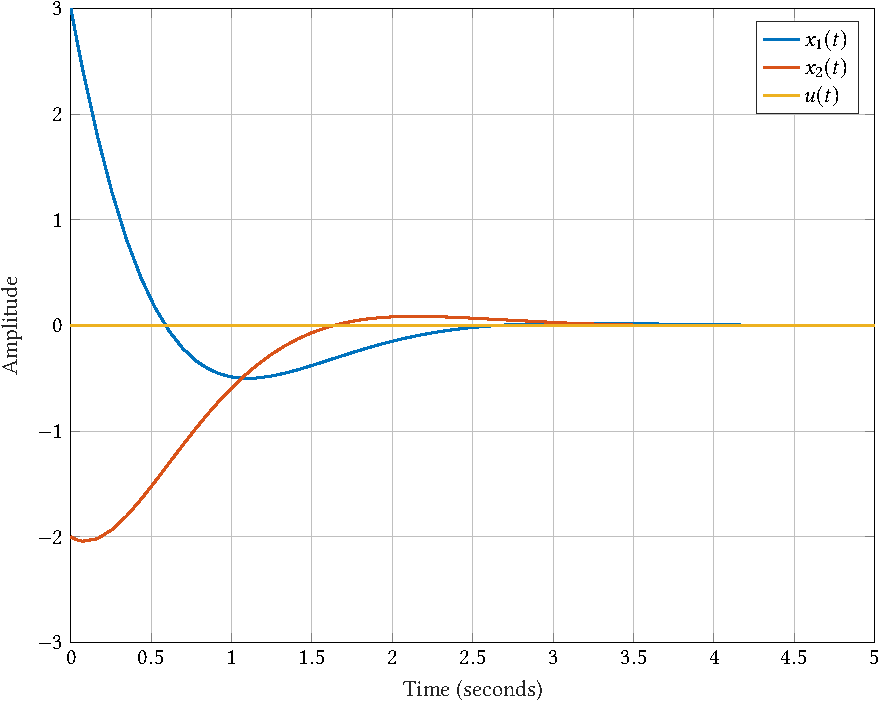
\includegraphics[width=0.9\textwidth]{figures/gcc_lmi3.pdf}
    \captionG{Σύστημα με αβεβαιότητες, \( r_1 = -1, r_2 = -1, p_1 = -1 \)}
    \label{fig:gcc_lmi3}
\end{figure}

Ο κώδικας για το παράδειγμα της μεθόδου ελαχιστοποίησης εγγυημένου κόστους
με τις γραμμικές ανισότητες πινάκων, για την περίπτωση με αβεβαιότητες στον
πίνακα των καταστάσεων και πίνακα ελέγχου παρατίθεται παρακάτω.
\eng{\lstinputlisting[language=Matlab]{src/gcc_lmi.m}}
